% Integer lattice with x+y<=4: solid triangle border, dashed inner grid, 15 dots.
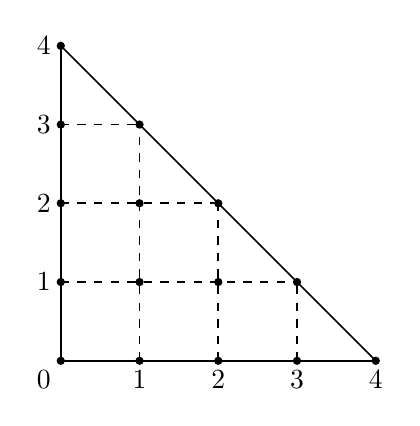
\begin{tikzpicture}[x=1cm,y=1cm,line width=.6pt,font=\normalsize]
% Interior dashed grid (horizontal and vertical up to hypotenuse x+y=4)
\draw[dashed] (0,1)--(3,1);
\draw[dashed] (0,2)--(2,2);
\draw[dashed] (0,3)--(1,3);
\draw[dashed] (1,0)--(1,3);
\draw[dashed] (2,0)--(2,2);
\draw[dashed] (3,0)--(3,1);
% Solid triangle border (no arrows in original)
\draw (0,0)--(4,0);
\draw (0,0)--(0,4);
\draw (0,4)--(4,0);
% Lattice dots at integer points with x+y<=4
\foreach \x/\y in {0/0,1/0,2/0,3/0,4/0,0/1,1/1,2/1,3/1,0/2,1/2,2/2,0/3,1/3,0/4} {\fill (\x,\y) circle (1.5pt);}
% Axis numbers
\node[below left] at (0,0) {$0$};
\node[below] at (1,0) {$1$};
\node[below] at (2,0) {$2$};
\node[below] at (3,0) {$3$};
\node[below] at (4,0) {$4$};
\node[left] at (0,1) {$1$};
\node[left] at (0,2) {$2$};
\node[left] at (0,3) {$3$};
\node[left] at (0,4) {$4$};
\end{tikzpicture}
